\title{Generalizations of Fourier analysis}

When I first learned about Fourier series and integrals, I hated it
because it seemed like a collection of many ad-hoc definitions,
formally related but very different.

To have a wider view of the subject, it helped me to realize that
Fourier series and integrals are a particular case of not one,
but many different constructions.  Thus, they can be generalized in
widely different directions, leading to differently flavored views of
the original theory.

\newcommand{\R}{\mathbf{R}}
\newcommand{\Z}{\mathbf{Z}}
\newcommand{\Q}{\mathbf{Q}}
\newcommand{\C}{\mathbf{C}}
\newcommand{\U}{\mathbf{U}}
\newcommand{\ud}{\mathrm{d}}

\begin{itemize}
	\item First you have the {\bf four classic cases} that you may learn in
		school: Fourier series of periodic functions, Fourier
		transforms of integrable functions, the discrete-time Fourier
		transform and the discrete Fourier transform.
		These four classic cases are fundamental and you must learn
		their definition and properties by heart.
	\item Then, you learn {\bf sampling theory} and you see that
		some of the classic cases may be obtained from the others.
		For example, the discrete Fourier transform can be
		considered a particular case of Fourier series of a
		periodic function.
		These relationships can be neatly arranged in the
		so-called Fourier-Poisson cube.
	\item Later, you learn {\bf distribution theory}, that
		provides a common framework for signals and their
		samples using Dirac combs.  Thus each of the four
		classic cases arises as a particular case of the
		Fourier transform of tempered distributions on the
		real line.
	\item A very different generalization is given by {\bf
		Pontryagin duality}.  This begins by realizing that
		the domain of definition of each classic case has
		always the structure of a commutative group ($\R$,
		$\Z$, $S^1$ or $\Z/N\Z$).  Then, Pontryagin duality
		provides a general construction for Fourier analysis
		on commutative groups, and the four classic cases
		are particular cases of it.
	\item By relaxing the condition of commutativity, you get {\bf
		non-commutative harmonic analysis}.  The case of a compact
		non-commutative group is described completely by the
		Paley-Wiener theorem, and the general non-compact
		non-commutative case is a large problem in representation
		theory, of which much is known; especially if the group has
		some additional structure (semisimple, solvable).
	\item The next step is {\bf harmonic analysis on homogeneous
		spaces}.  It turns out that the group structure is not
		essential, and you can do almost everything just by having a
		group acting on your space, which need not be itself a group.
		For example, the sphere~$S^2$ is not a group, but there is the
		group of~$3D$ rotations acting over it, and this leads to
		spherical harmonics.
	\item Finally there is {\bf spectral geometry}, also called the
		spectral analysis of the Laplace-Beltrami operator.  If your
		space is just a potato (a compact Riemannian manifold), there
		is no group whatsoever acting on it, but you still have a
		Laplace-Beltrami operator, it has a discrete spectrum, and you
		can do the analogue of Fourier series on it.  A large part of
		the classic results of Fourier series extend to this case,
		except everything related to convolution---which is defined
		necessarily using the group structure.
\end{itemize}

Thus, what happens when you ask a mathematician, \emph{``what is
Fourier analysis?''}~?

If they are a {\bf real analyst}, they will say that Fourier analysis
are a set of examples in the study of tempered distributions.

If they are an {\bf algebraist}, they will say that Fourier analysis
is a very particular case of one-dimensional representation theory.

If they are a {\bf geometer}, they will say that Fourier analysis is
a particular case of spectral geometry for trivial flat manifolds.

Finally, if you ask a {\bf complex analyst}, they will say that
Fourier series are just Taylor series evaluated on the unit circle.

And all of them will be right.



%We describe two common generalizations of elementary harmonic analysis:
%Pontryagin duality and Laplace-Beltrami spectral theory.  They lead to two
%different, but equivalent, definitions of spherical harmonics.

\section{The four classic cases}

The {\bf classic cases} of Fourier analysis are used to express an
arbitrary function~$f(x)$ as a linear combination of sinusoidal functions
of the form~$x\to e^{i\xi x}$.  There are {\bf four} cases, depending on
the space where~$x$ belongs.

\subsection{Fourier series}

Any periodic function
$$
f:S^1\to\R
$$
can be expressed as a numerable linear combination of sinusoidal waves. This is
called the \emph{Fourier series} of $f$
$$
	f(\theta) = \sum_{n\in\Z} a_n e^{in\theta}
$$
and the coefficients $a_n$ are computed as integrals of $f$
$$
	a_n = \frac{1}{2\pi}\int_{S^1} f(\theta) e^{-in\theta}
\mathrm{d}\theta
$$

%Parseval's theorem states that the function~$f$ and the
%coefficients~$a$ have the same energy:
%$$
%\sum_{n\in\Z}|a_n|^2 =
%\frac{1}{2\pi}\int_{S^1}|f(\theta)|^2\mathrm{d}\theta
%$$

\subsection{Fourier transform}

An arbitrary (integrable) function
$$
f:\R\to\R
$$
can be expressed as a linear combination of sinusoidal waves.  The
coefficients of this linear combination are called the \emph{Fourier
integral} of $f$, also known as Fourier transform or characteristic
function of $f$, depending on the context.  Thus,~$f$ is represented
as
$$
f(x) = \int_\R a(\xi) e^{i\xi x} \mathrm{d} \xi
$$
This is exactly analogous to the Fourier series above, but now the coefficients
$a$ of the linear combination are indexed by a continuous index
$\xi\in\mathbf{R}$ instead of a discrete index $n\in\mathbf{Z}$.  The values
of $a(\xi)$ can be recovered by integrating again the function $f$:
$$
a(\xi) = \frac{1}{2\pi}\int_\R f(x) e^{-i\xi x} \mathrm{d} x
$$
Notice that, even if their formulas look quite similar, the Fourier
series is not a particular case of the Fourier transform.  For
example, a periodic function is never integrable over the real line
unless it is identically zero.  Thus, you cannot compute the Fourier
transform of a periodic function.



\subsection{Discrete Fourier transform}

In the finite case, you can express any vector
\begin{equation}
(f_1, f_2, \ldots f_N)
\end{equation}
as a linear combination of "oscillating" vectors:
\begin{equation}
f_k = \sum_l a_l e^{\frac{2\pi}{N}ikl}
\end{equation}
This is called the \emph{discrete Fourier transform}.
The coefficients $a_l$ can be recovered by inverting the matrix $M_{kl} =
e^{\frac{2\pi}{N}ikl}$, which is unitary.  Thus
$$
a_l = \frac{1}{N}\sum_k f_k e^{-\frac{2\pi}{N}ikl}
$$

\subsection{Discrete-time Fourier transform}

Finally, if you have a doubly-infinite sequence:
\begin{equation}
\ldots,f_{-2},f_{-1},f_0,f_1,f_2,\ldots
\end{equation}
you can express it as a linear combination (integral) of sinusoidal functions
sampled at the integers, which is quite a thing:
\begin{equation}
f_n = \int_{S^1} a(\theta) e^{in\theta}
\mathrm{d}\theta
\end{equation}
The coefficients $a(\theta)$ of this infinite linear combination can be
recovered as a linear combination of all the values of $f$:
\begin{equation}
	a(\theta) = \frac{1}{2\pi}\sum_n f_n e^{-in\theta}
\end{equation}
Notice these two formulas are exactly the same as Fourier series, but
reversing the roles of~$a$ and~$f$.
This is an important symmetry.



\section{Pontryagin duality}

Pontryagin duality extracts the essence of the definitions of Fourier
series, Fourier integrals and discrete Fourier transforms.  The main idea is
that we have a \emph{spatial domain} $G$ and a \emph{frequency domain} $G^*$.
Then, any function defined on the spatial domain
\begin{equation}
f:G\to\mathbf{R}
\end{equation}
can be expressed as a linear combination of certain functions $E$, indexed by
the frequencies
\begin{equation}
f(x) = \int_{G^*} a(\xi) E(x,\xi) \mathrm{d} \xi
\end{equation}
Here the coefficients $a$ depend on the function $f$ but the functions $E$
depend only on the group $G$; they are called the \emph{characters} of $G$.
The coefficients $a$ can be found by computing integrals over the spatial
domain:
\begin{equation}
	a(\xi) = \int_G f(x) \overline{E(x,\xi)} \mathrm{d} \xi
\end{equation}
where the bar denotes complex conjugation.
Notice that these formulas include Fourier series, Fourier integrals, the
DFT and the DTFT as particular cases, according to the following table

\begin{tabular}{l|llll}
	 & space & freq. & analysis & synthesis \\
	\hline
	&
	$G$ &
	$G^*$ &
	$\displaystyle\widehat{f}(\xi)=\int_G f(x) \overline{E(\xi,x)}\ud x$ &
	$\displaystyle f(x)=\int_{G^*} \widehat{f}(\xi)E(\xi,x)\ud\xi$
	\\
	FS &
	$S^1$ &
	$\Z$ &
	$\displaystyle f_n =
			\frac{1}{2\pi}\int_0^{2\pi} f(\theta)e^{-in\theta}\ud\theta$ &
			%\frac{1}{2\pi}\int_{S^1} f(\theta)e^{-in\theta}\ud\theta$ &
	$\displaystyle f(\theta)=\sum_{n\in\mathbf{Z}} f_n
			e^{in\theta}$
	\\
	FT &
	$\R$ &
	$\R$ &
	$\displaystyle\widehat{f}(\xi)=\frac{1}{\sqrt{2\pi}}\int_\R f(x)e^{-i\xi x}\ud x$ &
	$\displaystyle f(x)=\frac{1}{\sqrt{2\pi}}\int_{\mathbf{R}} \widehat{f}(\xi)e^{i\xi x}\ud \xi$
	\\
	DFT &
	$\Z_N$ &
	$\Z_N$ &
	$\displaystyle\widehat{f}_k=\frac{1}{N}\sum_{n=0}^{N-1}f_n\,e^{-2\pi ikn/N}$ &
	$\displaystyle f_n=\sum_{k=0}^{N-1}\widehat{f}_k\,e^{2\pi ikn/N}$
	\\
	DTFT &
	$\Z$ &
	$S^1$ &
	$\displaystyle \widehat{f}(\theta)=\sum_{n\in\mathbf{Z}} f_n e^{-in\theta}$ &
	$\displaystyle f_n = \frac{1}{2\pi}\int_0^{2\pi}\widehat{f}(\theta)e^{in\theta}\ud\theta$
\end{tabular}

\subsection{Locally compact abelian groups}

A topological group is a group together with a topology compatible with the
group operation.  A morphism between two topological groups is a mapping
which is at the same time continuous and a group morphism.
Here we are interested in locally compact abelian groups (LCAG).  We
will denote the group operation by $x+y$, and the inverse of a group element
$x$ by $-x$.

The canonical example of LCAG is $\R^n$ with the usual topology and
the operation of sum of vectors.  Another example of LCAG is the
multiplicative group $\U$ of complex numbers of norm 1, which
topologically coincides with the unit circle $S^1$.  Other examples are any
finite abelian group with the discrete topology; or $\Z$, the
additive group of integers with the discrete topology.

The group $\U$ is very important in the following discussion.  It can
be denoted multiplicatively (by considering its elements as complex numbers),
or additively (by considering its elements as angles).  Both notations are
used henceforth, and they are linked by the relation
\[
e^{i\alpha}e^{i\beta}
=
e^{i(\alpha+\beta)}
\]


\subsection{Characters and the dual group}

Let $G$ be a LCAG.  A character of $G$ is a morphism from $G$ to
$\U$.  The set $G'$ of all characters of $G$ is a group (with the
operation of pointwise sum of mappings) and also a topological space (with the topology
of compact convergence).  It turns out that this group is locally compact,
thus it is a LCAG.  It is called the dual group of $G$.  There is a canonical
morphism between $G$ and its bidual, and it can be seen easily that this
morphism is injective.  The Pontryagin duality theorem states that $G$ is
isomorphic to its bidual.  Another result states that $G$ is compact if an
only if its dual is discrete.

For example, the dual group of $\R^n$ is itself.  The integers
$\Z$ and the unit circle $\U$ are dual to each other.
The dual of any finite group is isomorphic (though non-canonically) to
itself.

The action of a character $\xi\in G'$ over a group element $x\in G$ is
denoted by $E(\xi,x)$ or even $e^{i\xi x}$.  In the latter case, the complex
conjugate of $e^{i\xi x}$ is denoted by $e^{-i\xi x}$.  The exponential
notation is justified by the following properties, arising from the
definitions

\begin{itemize}
	\item $E(\xi,x)$ is a unit complex number, thus it has the form
	$e^{i\theta}$ for some real number $\theta$
	\item $E(\xi,x+y) = E(\xi,x)E(\xi,y)$, by the definition of character
	\item $E(\xi + \eta,x) = E(\xi,x)E(\eta,x)$, by the definition of dual
	group
\end{itemize}

\subsection{Haar measures}

Let $G$ be a LCAG.  A non-vanishing measure over $G$ which is invariant by
translations is called a Haar measure.  Haar's theorem states that there is a
single Haar measure modulo multiplication by positive constants.  Another
result states that $G$ is compact if and only if its total Haar measure (any
one of them) is finite.

For example, Lebesgue measure on $\R^n$ is a Haar measure.  The
counting measure of a discrete group is a Haar measure.

Given $G$, we fix a single Haar measure and we can talk about the spaces
$L^p(G)$.  The elements of this space are complex-valued functions such that
the $p$th power of their norm has finite integral with respect to Haar's
measure.  Notice that the set $L^p(G)$ does not depend on the actual choice
of normalization factor selected for the definition of the Haar measure.

\subsection{Fourier transform}

Now we can define a general notion of Fourier transforms, for functions
belonging to the space $L^1(G)$.  The Fourier
transform of a function
\begin{equation}
f:G\to\mathbf{C}
\end{equation}
is a function
\begin{equation}
\hat f:G'\to\mathbf{C}
\end{equation}
defined by
\begin{equation}
\hat f(\xi) = \int_G f(x) e^{-i\xi x}\mathrm{d} x
\end{equation}
Here $e^{-i\xi x}$ denotes the conjugate of the complex number
$e^{i\xi x}=E(\xi,x)$.  The inverse transform of a function defined on $G'$ is defined similarly, but
without the conjugate:
\begin{equation}
\check f(x) = \int_{G'} f(\xi) e^{i\xi x}\mathrm{d} \xi
\end{equation}

Note that these definitions require selecting Haar measures on $G$
and $G'$ (this amounts to fixing two arbitrary constants).

\subsection{Harmonic analysis on locally compact abelian groups}

So far we have just given definitions: LCAG, characters, dual group, Haar
measure, and Fourier transform.  Now it is time to recover the main results
of harmonic analysis.

The first result is the {\bf Fourier inversion theorem} for $L^1(G)$, which
states that the inverse transform is actually the inverse, for an appropriate
choice of scaling of the Haar measures on $G$ and $G'$.  Such a pair of
measures are called harmonized, or dual to each other.  In the following,
when we state a result involving integrals on $G$ and $G'$ we will always
assume that the Haar measures are harmonized.

The second result is the {\bf energy conservation theorem} for $L^2(G)$,
which states that, when $f$ and $\hat f$ are square-integrable, we have
\begin{equation}
\|f\|_{L^2(G)}
=
\|\hat f\|_{L^2(G')}
\end{equation}
Particular cases of this theorem are the formulas of Parseval, Plancherel,
etc.
The energy conservation theorem is needed to extend by continuity the
definition of Fourier transforms to $L^2(G)$

The third result is the {\bf convolution theorem}.  First notice that the
group structure allows to define the convolution of any two functions on
$L^1(G)$:
\begin{equation}
[f*g](x) = \int_G f(y)g(x-y)\mathrm{d} y
\end{equation}
Now, the convolution theorem says that the Fourier transform takes
convolution to point-wise multiplication
\begin{equation}
\widehat{f*g} = \hat f \hat g
\end{equation}

There is a long list of results, that can be found elsewhere.  Let us mention
a last one.  The dual group $G'$ is itself a LCAG, so it has a Fourier
transform in its own right.  This mapping is the $L^2$ adjoint of the inverse
Fourier transform defined from $G$.

Finally, notice that in the case of finite groups all these results are
trivial and they amount to elementary linear algebra.  In the continuous case
they are not trivial, mainly because we don't have an identity element for
the convolution (e.g., the dirac delta function), and to prove the results
one has to resort to successive approximations of the identity.

The sequence of proofs typically starts by the convolution theorem,
which is used to prove the conservation of energy for functions that
belong to~$L^1\cap L^2$, then to extend by density the definition of
the Fourier transform to~$L^2$ and finally to prove the inversion
theorem.  Except the definition of the Haar measure and the
approximation of the identity, which are particular construction, the
rest of the proofs are identical to the corresponding proofs for the
case of Fourier transforms on the real line.  You just have to check
that all the steps on the proof make sense in a group.


\section{Sampling theory}

Pontryagin duality gives an unified treatment of the four classic
cases in Fourier analysis: you are always doing exactly the same
thing, but in different groups.  However, it does not say anything
about the direct relationship between them.  For example, a Fourier
series where all but a finite number of the coefficients is zero can
be represented as a vector of length~$N$.  Does it have any
relationship with the discrete Fourier transform on~$\Z_N$?  The
answer is~\emph{yes}, and it is the main result of sampling theory.

Let us start with precisely this case.  Suppose that we have a
periodic function~$f(\theta)$ whose Fourier series is finite (this is
called a trigonometric polynomial).  For
example,
$$
f(\theta)=\sum_{n=0}^{N-1} f_ne ^{in\theta}
$$
Now, we can do \emph{three} different things with this object.  {\bf
One}, we can express the coefficients~$f_n$ as integrals of~$f$:
$$
f_n = \frac{1}{2\pi}\int_0^{2\pi} f(\theta)e^{-in\theta}\ud\theta
$$
{\bf Two}, we can consider the vector of
coefficients~$(f_0,\ldots,f_{N-1})$ and compute its inverse DFT
$$
\check{f}_k = \sum_{n=0}^{N-1} f_n\,e^{2\pi i nk/N}
$$
and {\bf three}, just for fun, we can evaluate the function~$f$
at~$N$ points evenly spaced along its period
$$
f\left(\frac{2\pi\cdot 0}{N}\right),
f\left(\frac{2\pi\cdot 1}{N}\right),
f\left(\frac{2\pi\cdot 2}{N}\right),
\ldots
f\left(\frac{2\pi(N-1)}{N}\right)
$$

These three operations are, a-priori, unrelated.  At least,
Pontryagin duality does not say anything about them, you are
working with different groups~$S^1$ and~$\Z_N$ that have nothing to
do with each other.

However, a number of very funny coincidences can be observed:

\begin{enumerate}
	\item The $k$-th sample~$f\left(\frac{2\pi k}{N}\right)$ equals
		$$
		\sum_{n=0}^{N-1}f_n\,e^{2\pi ikn/N}
		$$
		which is exactly~$\check{f}_k$
	\item Thus, the vector of samples of the polynomial~$f$ is the
		IDFT of the vector of coefficients
	\item Correspondingly, the vector of~$N$ coefficients of the
		polynomial~$f$ is the DFT of the vector of~$N$ uniform samples
		of~$f$ between~$0$ and~$2\pi$.
	\item In other words, the complete Fourier series of~$f$ can be
		obtained by evaluating the function~$f$ at~$N$ points.
	\item If you approximate the integral that evaluates~$f_n$
		from~$f$ as a sum of~$N$ step functions obtained by
		sampling~$f$, the computation is exact.
\end{enumerate}

All these results lie at the core of sampling theory.
They provide a beautiful, analog interpretation of the definition of
the discrete Fourier transform.  In fact, regardless of the
definition using group characters, we could have defined the discrete
fourier transform using these results! (property 3 above).

The {\bf sampling theorem} takes many different forms, but it always
amounts to a conservation of information, or conservation of degrees of
freedom.  Thus, the properties above can be rephrased as
\begin{enumerate}
	\item Evaluating a trigonometric polynomial of~$N$ coefficients
		at~$N$ points is a linear map~$\C^N\to\C^N$
	\item This linear map is invertible if and only if the points are different
		(thus, the function can be exactly recovered from~$N$ of its samples)
	\item If the points are uniformly distributed, this linear map is
		the discrete Fourier transform
\end{enumerate}

The second statement is often called the sampling theorem.  The
condition that to recover a polynomial of~$N$ coefficients
requires~$N$ samples is called the Nyquist condition.  Since
it is natural to consider trigonometric polynomials of the form
$$
P(\theta)=\sum_{n=-N/2}^{N/2} p_n\,e^{in\theta}
$$
the Nyquist condition is often stated as \emph{the sampling rate must
be at least the double of the maximal frequency}.

We have thus related Fourier series with the~$N$-dimensional DFT, via
the operation of sampling at~$N$ point.  The reasoning is finite and
mostly trivial.  There are a lot more correspondences between the
four classic cases.  For example, Shannon-Whittaker interpolation
relates the Fourier transform with the discrete-time Fourier
transform: if the support of~$\hat f$ lies inside the
interval~$[-\pi,\pi]$, then~$f$ can be recovered exactly by the
values~$f(\Z)$.  A different construction relates Fourier transforms
and Fourier series: if we have a rapidly decreasing function~$f(x)$,
we can build a~$2\pi$-periodic function by folding it:
$$
\tilde f(\theta)=\sum_{n\in\Z} f(\theta+2\pi n)
$$
and the Fourier series of~$\tilde f$  and the Fourier transform
of~$f$ are closely related.

All these relationships between the four classic cases are neatly
encoded in the Fourier-Poisson cube, which is an awesome commutative
diagram:

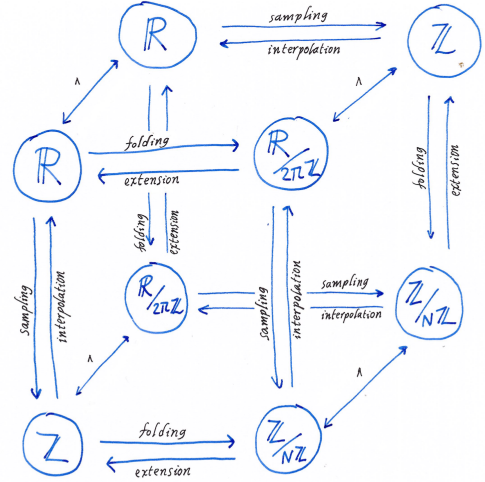
\includegraphics{i/hfpcube.png}



\section{Distributions}

Notice that most of sampling theory can be done without recourse to
distributions.  Indeed, Shannon, Nyquist, Whittaker, Borel, all
stated and proved their results way before the invention of
distributions.  Nowadays, distribution theory provides a satisfying
framework to state all the classic sampling results in a unified
form.  It is difficult to judge which method is simpler, because the
classic sampling results all have elementary proofs, while the
detailed definition of tempered distributions is a bit involved.
It is better to be familiar with both possibilities.

In {\bf classical sampling theory}, you sample a continuous
function~$f:\R\to\C$ by evaluating it at a discrete set of points,
for example~$\Z$, thus obtaining a sequence of
values~$\ldots,f(-2),f(-1),f(0),f(1),f(2),\ldots$, which can be
interpreted as a function~$\tilde f:\Z\to\C$.  Thus, the sampling
operation is a mapping between very different spaces: from the
continuous functions defined over~$\R$ into the functions defined
over~$\Z$.

When you perform {\bf sampling using distributions}, you sample a
smooth function~$f$ by multiplying it by a Dirac comb.  Thus,
the sampling operation is linear a mapping between subspaces of the same
space: tempered distributions.

\subsection{Distributions: overview}

Distributions are an extension of functions just like the real
numbers~$R$ are an extension of the rationals~$Q$.  Most of the
operations that can be done with~$Q$ can be done with~$R$, and then
some more.  Still, there is a price to pay: there are some
operations that only make sense on the smaller set.  For example,
while the~``denominator'' function on~$\Q$ cannot be extended
meaningfully to~$\R$, the elements of~$\R$ can not be enumerated like
those of~$\Q$, etc.  However, if you want to work with limits, the
space~$\Q$ is mostly useless and you need~$\R$.

There are a few spaces of distributions.  The three most famous are
\begin{itemize}
	\item $\mathcal{D}'$ the space of all distributions
	\item $\mathcal{S}'$ the space of tempered distributions
	\item $\mathcal{E}'$ the space of compactly supported distributions
\end{itemize}

Each of these spaces is a huge generalization of an already very large
space of functions:
\begin{itemize}
	\item $\mathcal{D}'$ contains all functions of~$L^1_{loc}$
	\item $\mathcal{S}'$ contains all functions of~$L^1_{loc}$ that
		are slowly growing (bounded, or going to infinity at a polynomial
		rate)
	\item $\mathcal{E}'$ contains all compactly supported integrable
		functions
\end{itemize}
Here~$L^1_{loc}$ denotes the set of locally integrable functions,
that is, complex-valued functions such that~$\int_K|f| <+\infty$ for
any compact~$K$.

These are the properties that we earn with respect to the original
spaces:
\begin{itemize}
	\item Most operations on functions extend naturally to
		distributions: sums, product by scalars, product by a function,
		affine changes of variable
	\item Any distribution is infinitely derivable, and the derivative
		belongs to the same space
	\item Any distribution is locally integrable
	\item The Fourier transform is an isometry in the space of
		tempered distributions
	\item There is a very easy to use definition of limit of
		distributions
\end{itemize}

And these are the prices to pay for the daring:
\begin{itemize}
	\item You cannot evaluate a distribution at a point
	\item You cannot multiply two distributions
	\item There is no way to define a norm in the vector space of
		distributions
\end{itemize}

\subsection{Distributions: definition}

There are several, rather different, definitions of distribution.
The most practical definition today seems to be as the topological
duals of spaces of test functions:

\begin{itemize}
	\item $\mathcal{D}$ the space of all $\mathcal{C}^\infty$
		functions of compact support
	\item $\mathcal{S}$ the space of all rapidly
		decreasing~$\mathcal{C}^\infty$ functions
	\item $\mathcal{E}$ the space of all~$\mathcal{C}^\infty$
		functions
\end{itemize}

Notice that~$\mathcal{D}$ and~$\mathcal{E}$ make sense for functions
defined over an arbitrary open set, but~$\mathcal{S}$ only makes
sense on the whole real line.

The only problem with this is that the topologies on these spaces of
test functions are not trivial to construct.  For example, there is
no natural way to define useful norms on these spaces.  Thus,
topologies need to be constructed using families of seminorms, or by
other means (in the case of~$\mathcal{D}$).  This is out of the scope
of this document, but it's a standard construction that can be easily
found elsewhere (e.g., Gasqued-Witomski).

The crucial topological property that we need is the definition of
{\bf limit of a sequence of distributions}.  We say that that a
sequence~$T_n$ of distributions converges to a distribution~$T$ when
$$
T_n(\varphi)\to T(\varphi)\qquad\textrm{for any test function }\ \varphi
$$
Thus, the limit of distributions is reduced to the limit of scalars.
A sequences of distributions is convergent if and only if it is
``pointwise'' convergent.  This is much more simple than the case of
functions, where there are several different and incompatible notions
of convergence.

A distribution is, by definition, a linear map on the space of test
functions.  The following notations are common for the result of
applying a distribution~$T$ to a test function~$\varphi$:
$$
T(\varphi)
\quad=\quad
\left<T,\varphi\right>
\quad=\quad
\int T\varphi
\quad=\quad
\int T(x)\varphi(x)\ud x
$$
The last notation is particularly insidious, because for a generic
distribution,~$T(x)$ does not make sense.  However, it is an abuse of
notation due to the following lemma:

{\bf Lemma.}  Let~$f$ be a locally integrable function (slowly
growing, or compactly supported).  Then the linear map
$$
T_f : \varphi\mapsto\int f(x)\varphi(x)\ud x
$$
is well-defined and continuous on~$\mathcal{D}$ (or~$\mathcal{S}$,
or~$\mathcal{E}$).  Thus it is a distribution.

The lemma says that any function can be interpreted as a
distribution.
This is very important, because {\bf all} the subsequent
definitions on the space of distributions are crafted so that, when
applied to a function they have the expected effect.

For example, the {\bf derivative of a distribution}~$T$ is defined by
$$
\left<T',\varphi\right>
:=
\left<T,-\varphi'\right>
$$
Two observations: (1) this definition makes sense, because~$\varphi$
is always a~$\mathcal{C}^\infty$ function, and so is~$-\varphi'$.
And (2) this definition extends the notion of derivative when~$T$
corresponds to a derivable function~$f$.  We write
$$
T_{f'}= {T_f}'
$$
to indicate that the proposed definition is compatible with the
corresponding construction for functions.

A similar trick is used to extend the shift~$\tau_a$, scale~$\zeta_a$ and
symmetry~$\sigma$ of functions (where~$a>0$):
\begin{eqnarray*}
	\tau_a f(x) &:= f(x-a) \\
	\zeta_a f(x) &:= f(x/a) \\
	\sigma f(x) &:= f(-x) \\
\end{eqnarray*}
to the case of distributions:
\begin{eqnarray*}
	\left<\tau_a T,\varphi\right> &:= \left<T,\tau_{-a}\varphi\right> \\
	\left<\zeta_a T,\varphi\right> &:= \left<T,a^{-1}\zeta_{a^{-1}}\varphi\right> \\
	\left<\sigma T,\varphi\right> &:= \left<T,\sigma\varphi\right> \\
\end{eqnarray*}
and the compatibility can be checked by straightforward change of
variable.

After regular functions, the most important example of distribution
is the {\bf Dirac delta}, defined by~$\delta(\varphi):=\varphi(0)$.
In the habitual notation we write
$$
\int\delta(x)\varphi(x)\ud x = \varphi(0)
$$
because this form is very amenable to changes of variable.
An equivalent definition is~$\delta(x)=H'(x)$ where~$H$ is the
indicator function of positive numbers.  This makes sense because~$H$
is locally integrable, and its derivative is well-defined in the
sense of distributions.  The Dirac delta belongs to all three
spaces~$\mathcal{D}'$, $\mathcal{S}'$ and $\mathcal{E}'$.

Using Diracs, we can define many other distributions, by applying
shifts, derivatives, and vector space operations.  For example, the
{\bf Dirac comb} is defined as
$$
\Xi(x)=\sum_{n\in\Z}\delta(x-n)
$$
where the infinite series is to be interpreted as a limit.  This is
well-defined in~$\mathcal{D}'$ (where the sum is finite due to the
compact support of the test function)
and~$\mathcal{S}'$ (where the series is trivially convergent due the
rapid decrease of the test function) but not on~$\mathcal{E}'$ (where
the series is not necessarily convergent for arbitrary test
functions, for example~$\varphi=1\in\mathcal{E}$).

We can do other crazy things, like~$\sum_{n\ge 0}\delta^{(n)}(x-n)$,
which is also well defined when applied to a test function.  But we
cannot do everything.  For example~$\sum_{n\ge 0}\delta^{(n)}(x)$ is
not well defined, because there is not a guarantee that the sum of
all derivatives of a test function at the same point converges.

\subsection{Fourier transform of distributions}

How to define the Fourier transform of a distribution?
We need to find a definition that extends the definition that we
already have for functions, thus~$\widehat{T_f}=T_{\widehat{f}}$.
It is easy to check that the definition
$$
\left<\widehat{T},\varphi\right>
:=
\left<T,\widehat{\varphi}\right>
$$
does the trick, because it corresponds to Plancherel Theorem when~$T$
is a locally integrable function.

However, notice that this definition does not make sense
in~$\mathcal{D}'$:  if~$\varphi\in\mathcal{D}$, then it has compact
support, so its Fourier transform does not,
thus~$\widehat{\varphi}\not\in\mathcal{D}$.

The space~$\mathcal{S}$, called the Schwartz space, has the beautiful
property of being invariant by Fourier transforms.  Indeed, the Fourier
transform, with appropriate normalization constants, is an~$L^2$
isometry on~$\mathcal{S}$.  Thus, tempered distributions are the
natural space where to perform Fourier transforms.

Now, we can compute the Fourier transform, in the sense of
distributions, of many functions!  For example, what is the Fourier
transform of the function~$f(x)=1$?  This function is a temperate
distribution, so it must have a Fourier transform, doesn't it?
Indeed it does, and it can be easily found from the definitions:
$$
\left<\widehat{1},\varphi\right>
=
\left<1,\widehat{\varphi}\right>
=
\int\widehat{\varphi}(x)\ud x
=
\frac{1}{\sqrt{2\pi}}\varphi(0)
$$
So, the Fourier transform of a constant is a Dirac!

By combining this result with the derivatives we can compute the
Fourier transform of polynomials.  For example~$f(x)=x^2$ has the
property that~$f''$ is constant, thus~$\widehat{f''}$ is a Dirac, and
then~$\widehat{f}$ is the second derivative of a Dirac.


\subsection{Sampling with Diracs}

Can we compute the Fourier transform of~$f(x)=e^x$ ?  No, because it
is not a slowly growing function, and it does not correspond to any
tempered distribution.

However, the function~$f(x)=e^{ix}$ is actually slowly growing (it is
bounded), so it has a Fourier transform as a tempered Distribution
that is~$\widehat{f}(\xi)=\delta(\xi-1)$.  Using trigonometric
identities, we find the Fourier transforms of~$\sin$ and~$\cos$,
which are also sums of Diracs:

\begin{eqnarray*}
	\widehat{\cos}(\xi) &=\frac{\delta(x-1)+\delta(x+1)}{2} \\
	\widehat{\sin}(\xi) &=\frac{\delta(x-1)-\delta(x+1)}{2i} \\
\end{eqnarray*}

And, as we would say in Catalan, \emph{the mother of the
eggs}\footnote{``La mare dels ous'', or in french ``où il gît le
lièvre''.  I do not know a similarly colorful expression in english}: the
Fourier transform of a Dirac comb is another Dirac comb.  I don not
know how to prove this by combining the identities above, but it has
a simple proof by expressing the Dirac comb as the derivative of a
sawtooth function and applying it to a test function.
$$
\textrm{(typeset the computation)}
$$

\section{Spectral geometry}

Spectral theory provides a brutal generalization of a large part of
Fourier analysis.  We do away with the group structure (and thus with
the possibility to have convolutions, which are based on the action
of the group).  In exchange, we need to work inside a compact space,
endowed by a Riemannian metric.  For example, a compact sub-manifold
of Euclidean space.  The canonical example is~$S^1$, that in
the classical case leads to Fourier series.  Here, we recover all
the results of Fourier series (except those related to periodic
convolution) for functions defined on our manifold.

Let~$M$ be a compact Riemannian manifold (with or without boundary), and
let~$\Delta$ be its Laplace-Beltrami operator, defined
as~$\Delta=*d*d$, where~$d$ is the exterior derivative (which is independent
of the metric) and~$*$ is the Hodge duality between~$p$-forms
and~$d-p$-forms (which is defined using the metric).

The following are standard results in differential geometry (see e.g.
Warner's book chapter
6~\url{https://link.springer.com/content/pdf/10.1007\%2F978-1-4757-1799-0_6.pdf})

\begin{itemize}
	\item[(1)] There is a sequence of~$\mathcal{C}^\infty(M)$
		functions~$\varphi_n$ and positive
		numbers~$\lambda_n\to\infty$ such that
		$$\Delta\varphi_n=-\lambda_n\varphi_n$$
	\item[(2)] The functions~$\varphi_n$, suitably normalized, are an
		orthonormal basis of~$L^2(M)$.
\end{itemize}

These results generalize Fourier series to an arbitrary smooth manifold~$M$.
Any square-integrable function~$f:M\to\R$ is written uniquely as
$$f(x)=\sum_nf_n\varphi_n(x)$$ and the coefficients~$f_n$ are computed by
$$f_n=\int_Mf\varphi_n.$$  Some particular cases are the habitual Fourier and
sine bases (but not the cosine basis), bessel functions for the disk, and
spherical harmonics for the surface of a sphere.

\begin{tabular}{lccr}
	&$M$ & $\varphi_n$ & $-\lambda_n$ \\
	\hline
	interval & $[0,2\pi]$ & $\sin\left(\frac{nx}{2}\right)$ & $n^2/4$ \\
	circle & $S^1$ & $\sin(n\theta),\cos(n\theta)$ & $n^2$ \\
	square & $[0,2\pi]^2$ &
	$\sin\left(\frac{nx}{2}\right)\sin\left(\frac{m\theta}{2}\right)$ &
	$\frac{n^2+m^2}{4}$ \\
	torus & $(S^1)^2$ & $\sin(nx)\sin(my),\ldots$ & $n^2+m^2$ \\
	disk & $|r|\le1$ & $\sin,\cos(n\theta)J_n(\rho_{m,n}r)$ &
	$\rho_{m,n}$ roots of~$J_n$ \\
	sphere & $S^2$ & $Y^m_l(\theta,\varphi)$ & $l^2+l$
\end{tabular}

The eigenfunctions~$\varphi_n$ are called the vibration modes of~$M$, and the
eigenvalues~$\lambda_n$ are called the (squared) fundamental frequencies of~$M$.

Several geometric properties of~$M$ can be interpreted in terms of the
Laplace-Beltrami spectrum.  For example, if~$M$ has~$k$ connected components,
the first~$k$ eigenfuntions will be supported successively on each connected
component.  On a connected manifold~$M$, the first vibration mode can be
taken to be positive~$\varphi_1\ge0$, thus all the other modes have
non-constant signs (because they are orthogonal to~$\varphi_1$).  In
particular, the sign of~$\varphi_2$ cuts~$M$ in two parts in an optimal way,
it is the Cheeger cut of~$M$, maximizing the perimeter/area ratio of the cut.

The zeros of~$\varphi_n$ are called the nodal curves (or nodal sets) of~$M$,
or also the Chladni patterns.  If~$M$ is a subdomain of the plane, these
patterns can be found by cutting an object in the shape of~$M$, pouring a
layer of sand over it, and letting it vibrate by high-volume sound waves at
different frequencies.  For most frequencies, the sand will not form any
particular pattern, but when the frequency coincides with
a~$\sqrt{\lambda_n}$, the sand will accumulate over the set~$[\varphi_n=0]$,
which is the set of points of the surface that do not move when the surface
vibrates at this frequency.  In the typical case, the number of connected
components of~$[\varphi_n>0]$ grows linearly with~$n$, thus the
functions~$\varphi_n$ become more oscillating (less regular) as~$n$ grows.

Generally, symmetries of~$M$ arise as multiplicities of eigenvalues.
The Laplace-Beltrami spectrum~${\lambda_1,\lambda_2,\lambda_3,\ldots}$ is
closely related, but not identical, to the geodesic length spectrum, that
measures the sequence of lengths of all closed geodesics of~$M$.  The grand
old man of this theory is Yves Colin de Verdière, student of Marcel Berger.

Geometry is not in general a spectral invariant, but non-isometric manifolds
with the same spectrum are difficult to come by.  The first pair of distinct
but isospectral manifolds was wound in 1964 by John Milnor, in dimension 16.
The first example in dimension 2 was found in 1992 by Gordon, Webb and
Wolperd, and it answered negatively the famous question of Marc Kac ``Can you
hear the shape of a drum?'.
In 2018, we have many ways to construct discrete and continuous families of
isospectral manifolds in dimensions two and above.



% vim:set ts=3 sw=3 tw=69 filetype=tex spell spelllang=en:
